\documentclass[10pt]{article}
% \usepackage{geometry}
% \geometry{margin=0.2in}
% \usepackage[X2]{fontenc}
\usepackage[utf8]{inputenc}
% \usepackage[utf8x]{inputenc}

\nonstopmode
% \usepackage{minted}[cache=false]
\usepackage{graphicx} % Required for including pictures
\usepackage[figurename=Figure]{caption}
% \usepackage{float}    % For tables and other floats
\usepackage{amsmath}  % For math
\usepackage{amssymb}  % For more math
\usepackage{fullpage} % Set margins and place page numbers at bottom center
% \usepackage{paralist} % paragraph spacing
% \usepackage{subfig}   % For subfigures
%\usepackage{physics}  % for simplified dv, and 
% \usepackage{enumitem} % useful for itemization
% \usepackage{siunitx}  % standardization of si units
\usepackage{hyperref}
% \usepackage{mmacells}
% \usepackage{listings}
% \usepackage{svg}
% \usepackage{xcolor, soul}
\usepackage{bm}
% \usepackage{amsthm}  % For math
\usepackage{mathtools}

% \usepackage{setspace}
% \usepackage{listings}
% \usepackage{listings}
% \usepackage[autoload=true]{jlcode}
% \usepackage{pygmentize}



% \usepackage[margin=1.8cm]{geometry}
% \newcommand{\C}{\mathbb C}
% \newcommand{\D}{\bm D}
% \newcommand{\R}{\mathbb R}
% \newcommand{\Q}{\mathbb Q}
% \newcommand{\Z}{\mathbb Z}
% \newcommand{\N}{\mathbb N}
% \newcommand{\PP}{\mathbb P}
% \newcommand{\A}{\mathbb A}
% \newcommand{\F}{\mathbb F}
% \newcommand{\1}{\mathbf 1}
% \newcommand{\ip}[1]{\left< #1 \right>}
% \newcommand{\abs}[1]{\left| #1 \right|}
% \newcommand{\norm}[1]{\left\| #1 \right\|}

% \def\Tr{{\rm Tr}}
% \def\tr{{\rm tr}}
% \def\Var{{\rm Var}}
% \def\calA{{\mathcal A}}
% \def\calB{{\mathcal B}}
% \def\calD{{\mathcal D}}
% \def\calE{{\mathcal E}}
% \def\calG{{\mathcal G}}
% \def\from{{:}}
% \def\lspan{{\rm span}}
% \def\lrank{{\rm rank}}
% \def\bd{{\rm bd}}
% \def\acc{{\rm acc}}
% \def\cl{{\rm cl}}
% \def\sint{{\rm int}}
% \def\ext{{\rm ext}}
% \def\lnullity{{\rm nullity}}
% \DeclareSIUnit\clight{\text{\ensuremath{c}}}
% \DeclareSIUnit\fm{\femto\m}
% \DeclareSIUnit\hplanck{\text{\ensuremath{h}}}
% \usepackage[cache=false]{minted}

% \usepackage{ tipa }

% \DeclareUnicodeCharacter{2208}{\ensuremath{\in}}
% \DeclareUnicodeCharacter{2082}{\ensuremath{\phantom{}_2}}
% \DeclareUnicodeCharacter{03A3}{\ensuremath{\Sigma}}
% \DeclareUnicodeCharacter{03C0}{\ensuremath{\pi}}
% \DeclareUnicodeCharacter{03C3}{\ensuremath{\sigma}}
% \DeclareUnicodeCharacter{03C4}{\ensuremath{\tau}}
% \DeclareUnicodeCharacter{0394}{\ensuremath{\Delta}}



% \definecolor{mintedbackground}{rgb}{0.902, 0.929, 0.906}

% \definecolor{cambridgeblue}{rgb}{0.81, 0.9, 0.84}



% \sethlcolor{mintedbackground}
% \newcommand{\mathcolorbox}[1]{\colorbox{mintedbackground}{$\displaystyle #1$}}

% \lstdefinelanguage{julia}%
%   {morekeywords={abstract,break,case,catch,const,continue,do,else,elseif,%
%       end,export,false,for,function,immutable,import,importall,if,in,%
%       macro,module,otherwise,quote,return,switch,true,try,type,typealias,%
%       using,while},%
%    sensitive=true,%
% %    alsoother={$},%
%    morecomment=[l]\#,%
%    morecomment=[n]{\#=}{=\#},%
%    morestring=[s]{"}{"},%
%    morestring=[m]{'}{'},%
% }[keywords,comments,strings]%

% \lstset{%
%     language         = Julia,
%     basicstyle       = \ttfamily,
%     keywordstyle     = \bfseries\color{blue},
%     stringstyle      = \color{magenta},
%     commentstyle     = \color{ForestGreen},
%     showstringspaces = false,
% }

% $
\begin{document}
\begin{center}
	\hrule
	\vspace{.4cm}
	{\textbf { \large CDS DS 210 --- Programming Data Science}}
\end{center}
{\textbf{Name:}\ Emmy Blumenthal \hspace{\fill} Final Project Report\hspace{\fill}  \textbf{BU ID:} \ U87312711 \\
\textbf{Due Date:}\  Dec 15, 2022   \hspace{\fill} \textbf{Email:}\ emmyb320@bu.edu \ 
\vspace{.4cm}
\hrule

\begin{center}
	\Large 
	{
	\bf
	Implementing Karger's Algorithm on the Facebook Social Circles Graph Dataset
	}
\end{center}

\tableofcontents


\section{Karger's Algorithm and Minimum Cuts}

\subsection{Introduction to Karger's Algorithm}

Karger's algorithm is a well-known randomized algorithm for finding a minimum cut in an undirected graph.
In an undirected graph, a minimum cut is a partition of the vertices into two disjoint sets, such that the number of edges crossing the partition is minimized. In other words, a minimum cut is a way of dividing the vertices of the graph into two groups, such that the number of edges connecting the two groups is as small as possible.
The algorithm works by repeatedly contracting randomly-selected edges in the graph until only two vertices remain.
Karger's algorithm has a running time of $O(n^2m)$, where $n$ is the number of vertices and $m$ is the number of edges in the graph. Although the algorithm is simple and efficient, it is not guaranteed to find the minimum cut with high probability. However, the probability of finding the minimum cut can be increased by running the algorithm multiple times and taking the minimum cut found across all runs. Karger's algorithm has numerous applications in various fields, including network design, image segmentation, and data mining. It is an important tool in the field of graph theory and has been extensively studied and utilized in practice.

\urldef\wikiurl\url{https://commons.wikimedia.org/wiki/File:Single_run_of_Karger%E2%80%99s_Mincut_algorithm.svg#/media/File:Single_run_of_Karger’s_Mincut_algorithm.svg}

\begin{figure}[h!]
	\centering
	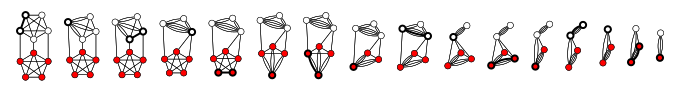
\includegraphics[width=0.8\linewidth]{wiki_karger.png}
	\caption{Karger's algorithm successfully identifying the minimum cut between sparsely connected complete graphs with five vertices.
	Image source: {\em Wikipedia} (\wikiurl)}
\end{figure}

\subsection{Nature of my Implementation of Karger's Algorithm}

In my implementation of Karger's algorithm, although the input of the function is an adjacency list, I represent the graph using a nested hashmap.
Specifically, each vertex is taken as a key in a hashmap whose associated value is another hashmap whose keys represents vertices to which it is connected and whose values are the multiplicity of connections between the vertices.
It is necessary to record the multiplicity of connections between the vertices so that I am able to sample uniformly over the set of contracted edges instead of sampling over the set of contracted vertices; this sampling is an essential part of the statistical properties of Karger's algorithm.
In order to represent contraction of edges, I also have a vector of integers which represent nodes that have been contracted into; this helps us specify which vertices have been deleted as part of edge contraction without having to iterate through a hashmap.
At each iteration, edge contraction is performed by randomly sampling a first node weighted by how many connections it has (including multiplicity), random sampling a second, connected node also weighted by how many connections it has to the already-sampled node (including multiplicity), dropping the first node from the list of un-contracted vertices, replacing all references in other nodes to the first node with a reference to the second node (including multiplicity), and moving all connections from the first node to connections from the second node (including multiplicity).
The final result of the algorithm is a vector of length two whose elements are vectors which contain integers representing the vertices on either side of the minimum cut.


\section{Relationship to Original Project Proposal}

In the originally-submitted project proposal, I proposed using the HCS (Highly Connected Subgraphs) clustering algorithm on a dataset of gene expressions in embryonic mouse brain cells; however, this project was computationally and temporally infeasible for two reasons: dependencies of the HCS algorithm and the size of the embryonic mouse brain cells dataset.

The HCS algorithm requires two substantial components whose implementations are non-trivial: finding minimum cuts and testing if an undirected subgraph is highly connected.
When I was setting out to implement the HCS algorithm, I began exploring algorithms for finding minimum cuts and quickly learned that exact algorithms are computationally expensive, so I decided to implement Karger's algorithm.
After attempting implementation, I repeatedly ran into errors and statistical subtleties (like dealing with multiplicity of connections).
As I neared successfully implementing Karger's algorithm, I realized that the dataset I was interested in had just over 1,000,000 vertices and dense connections, and preliminary tests led to estimates that computations of the algorithm would take at least a day to complete on my laptop.
I additionally regularly encountered integer overflow when recording the multiplicity of connections as the number of connections grows exponentially as edges become repeatedly contracted; in the current implementation, I use integers of type u128 to account for such larger numbers.
These issues caused me to search for a smaller dataset on the Stanford Network Analysis Project website on which I successfully implemented Karger's algorithm.
At the time I had implemented Karger's algorithm on the new dataset, I concluded that my implementation would satisfy the appropriate bounds of the project and that, given my other responsibilities, it would be temporally infeasible to proceed with implementing the entire HCS algorithm.
Therefore, I am turning in my current implementation of Karger's algorithm as my project.
In further work or as a personal project, I could use what I have implemented here as an essential component of the HCS algorithm.

\section{The Facebook Social Circles Graph Dataset}

\begin{figure}[h!]
	\centering
	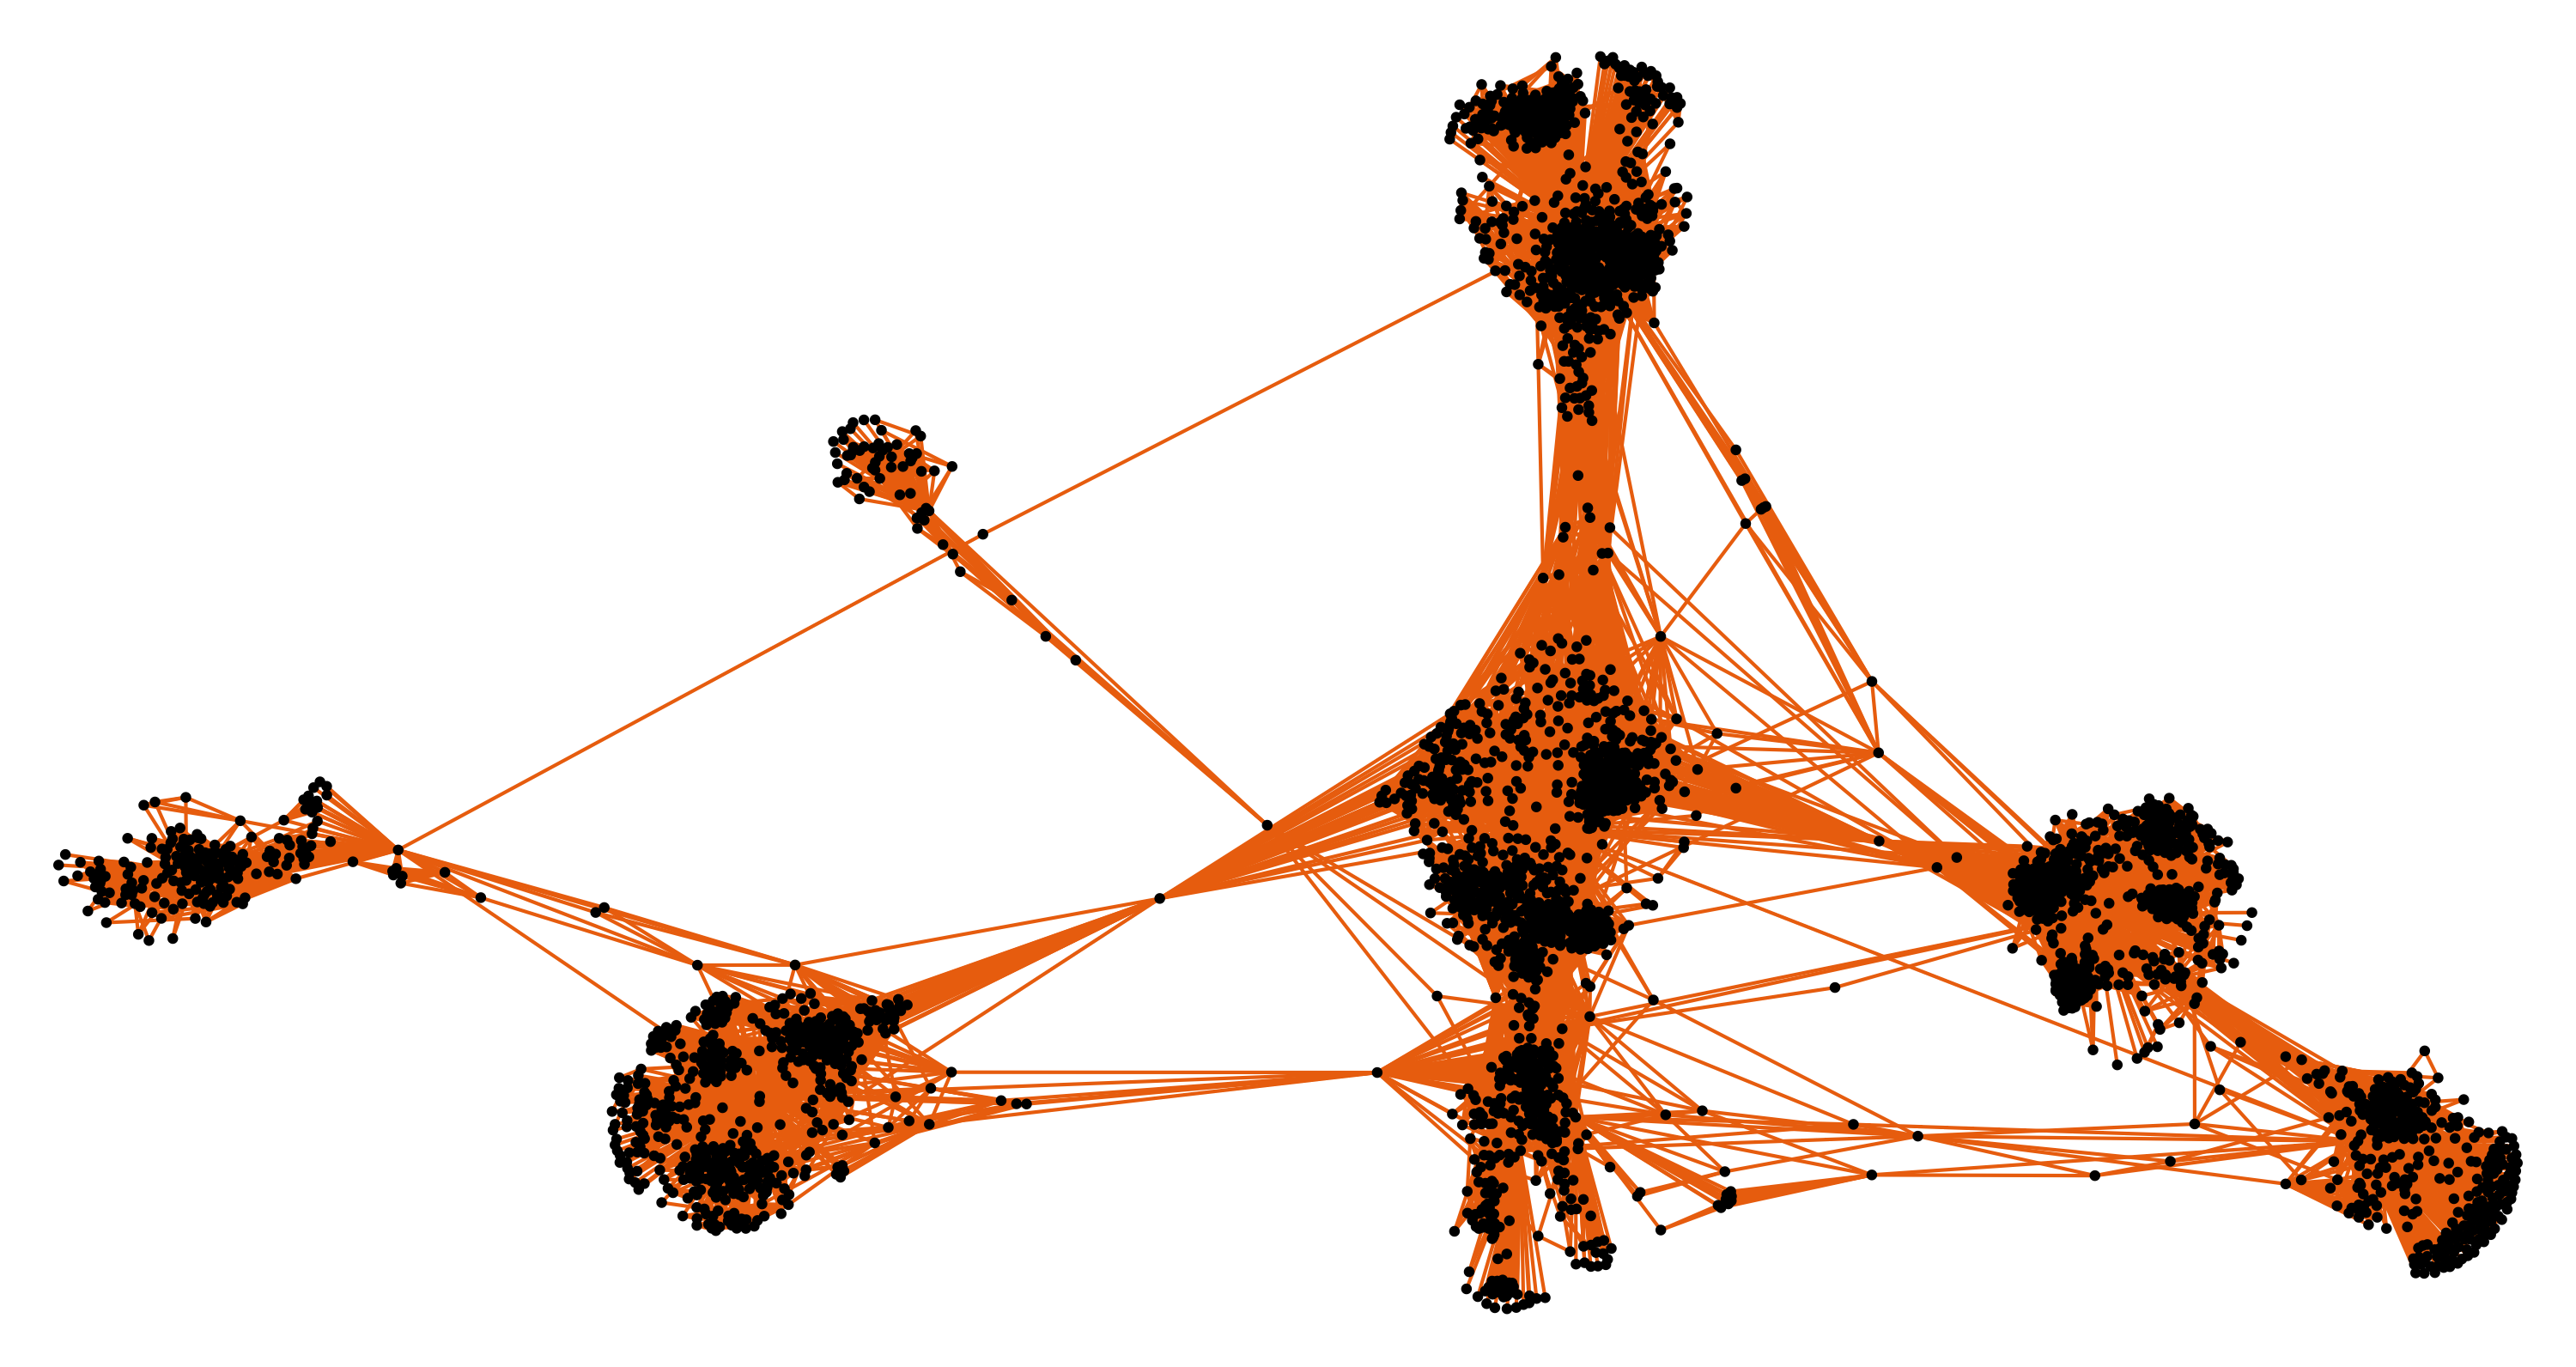
\includegraphics[width=0.7\linewidth]{mathematica_vis.png}
	\caption{Visualization of Facebook Social Circles graph dataset generated in {\em Mathematica} using the GraphPlot command.}
\end{figure}

The Stanford Network Analysis Project describes the Facebook Social Circles dataset (\url{https://snap.stanford.edu/data/ego-Facebook.html}):
\begin{quote}
	\em
	This dataset consists of 'circles' (or 'friends lists') from Facebook. Facebook data was collected from survey participants using this \href{https://www.facebook.com/apps/application.php?id=201704403232744}{Facebook app}. The dataset includes node features (profiles), circles, and ego networks. Facebook data has been anonymized by replacing the Facebook-internal ids for each user with a new value. 
\end{quote}
The dataset has 4039 nodes and 88234 edges, making it a reasonable size for my implementation and significantly smaller than the embryonic mouse brain cell \href{https://snap.stanford.edu/biodata/datasets/10023/10023-CC-Neuron.html}{dataset}.

\section{Performance and Results}

When running in release mode, the algorithm took approximately 18 seconds to run on the Facebook Social Circles dataset and returned data in the proper format: a vector of length two whose elements are vectors of integers.

\subsection*{A comment on tests}

As Karger's algorithm is randomized, it is not possible to get consistent results from a unit test for a non-trivial graph.
Therefore, I have only implemented one test, `cut\_a\_simple\_graph,' which checks that a contraction does indeed occur on a graph with two vertices and one edge.



% \section*{REPORT}

% % \url{https://snap.stanford.edu/biodata/datasets/10023/10023-CC-Neuron.html}

% The structure and differentiation of different cell types is a central question in biology and biophysics that has a history of combining epistemological questions (e.g., what is a cell type?) and quantitative methods.
% In this project, I will employ graph clustering methods to try to approach some of these questions from a basic level.
% I will investigate the `megascale cell-cell similarity network' from the Stanford network analysis project (\url{https://snap.stanford.edu/biodata/datasets/10023/10023-CC-Neuron.html}).
% Specifically, I will attempt to use a variety of graph clustering algorithms to find subgraphs/cliques of the similarity network which represent cells that are more similar to each other than other clusters of cells; an example algorithm I will implement is the highly connected subgraphs (HCS) clustering algorithm (\url{https://en.wikipedia.org/wiki/HCS_clustering_algorithm}).
% The relative success of the algorithm at finding independent clusters may tell me something about cell types.
% If clusters are sufficiently independent and there are many clusters, this tells us that cell types may be well-differentiated.
% On the other hand, if there are few clusters and/or it is difficult to find independent cliques/clusters, I might be able to conclude that cell types are difficult to differentiate using this method.

% If I am able to find sufficiently differentiated clusters, a next possible step would be implementing vertex centrality measures which may tell us which cells can serve as archetypes/representatives for their given cell type.
% These centrality measures would be implemented within the individual cell sub-graphs.
% Because individual cell's gene expressions often fluctuate significantly, it is likely that finding archetypal example cells may be difficult/infeasible.
% However, understanding the way in which various centrality methods may succeed or fail to identify only a few archetypes for each subgraph may provide some insights into how cell types could be defined and their structures of differentiation.
% Possible centrality measures that I may employ include closeness and eigenvector centrality.

% To accomplish this project, I will attempt to adhere to the following schedule:
% \begin{itemize}
% 	\item Week of Nov. 18: Download data and ensure that I can read data in the necessary formats (e.g., adjacency matrix, sparse representation)
% 	\item Week of Nov. 25: Give a first pass at implementing the HCS clustering algorithm; identify questions and errors that will need to be tackled after Thanksgiving break.
% 	\item Week of Dec. 2: Polish HCS clustering algorithm and seek support for persistent issues.
% 	Assess feasibility of implementing sub-graph centrality measures.
% 	\item Week of Dec. 9:
% 	If implementing sub-graph centrality measures is feasible given implemented HCS algorithm, implement two centrality measures and assess results relative to each other.
% 	If implementing sub-graph centrality measures is unsuccessful, attempt to implement a different sub-graph/clique clustering algorithm besides HCS.
% 	\item Week of Dec. 15:
% 	Finalize report on results; clean repository and source code.
% \end{itemize} 










\end{document}





